\chapter[HexPak/\GP Construction]{\GP and HexPak: A Variable-pitch,
  Dual-head IFU for the WIYN 3.5m Bench Spectrograph}
\label{chap:pak_build}
\epigraph{\fixspacing\emph{When the going gets weird, the weird turn
    pro}}{Raoul Duke}

% Leave space between title and quote or publication note.  This has often been
% 10cm for a quote and 8 cm for a reference, but this is really up to you.
%\vspace{8cm}

\vfill

\begin{flushright}
  \fixspacing
  \textit{A version of this chapter has previously appeared in\\
    \emph{Ground-based and Airborne Instrumentation for Astronomy IV. Proceedings of the SPIE}}\\
    \vspace{1ex}
    Wood, et. al. 2012. Volume 8446, article 84462W
\end{flushright}

%%%%%%%%%%%%%%%%%%%%%%%%%%%%%%%%%%%%%%%%%%%%%%%%%%%%%%%%%%%%% 
\begin{chabstract}
  We describe the design, construction, and expected performance of two new
  fiber integral field units (IFUs) --- HexPak and \GP --- for the WIYN 3.5m
  Telescope Nasmyth focus and Bench Spectrograph.  These are the first IFUs to
  provide formatted fiber integral field spectroscopy with simultaneous sampling
  of varying angular scales.  HexPak and \GP are in a single cable with a
  dual-head design, permitting easy switching between the two different IFU
  heads on the telescope without changing the spectrograph feed: the two heads
  feed a variable-width double-slit.  Each IFU head is comprised of a fixed
  arrangement of fibers with a range of fiber diameters.  The layout and
  diameters of the fibers within each array are scientifically-driven for
  observations of galaxies: HexPak is designed to observe face-on spiral or
  spheroidal galaxies while \GP is optimized for edge-on studies of galaxy
  disks.  HexPak is a hexagonal array of 2.9 arcsec fibers subtending a 40.9
  arcsec diameter, with a high-resolution circular core of 0.94 arcsec fibers
  subtending 6 arcsec diameter.  \GP is a 39 by 55 arcsec rectangular array
  with rows of fibers of increasing diameter from angular scales of 1.9 arcsec
  to 5.6 arcsec across the array.  The variable pitch of these IFU heads allows
  for adequate sampling of light profile gradients while maintaining the photon
  limit at different scales.
\end{chabstract}
\cleardoublepage

\section{Introduction}
\label{GPB:sec:intro}
HexPak and \GP are two new formatted fiber optic integral field units
(IFUs) for the WIYN 3.5m telescope Bench Spectrograph\footnotemark.
\footnotetext{The WIYN Observatory is a joint facility of the University of
  Wisconsin-Madison, Indiana University, Yale University, and the National
  Optical Astronomy Observatory.}  These two IFUs are unique because they are
the first formatted fiber IFUs to include multiple fiber diameters within the
same fiber head.  Including multiple fiber diameters allows each of these IFUs
to simultaneously sample different angular scales within the same observation.
The smaller fibers can gather light from higher surface brightness regions
(e.g.\ the core or midplane of a galaxy disk) while the larger fibers can
collect light from fainter, more diffuse regions (e.g.\ larger scale heights
or scale radii of a disk), thereby enabling high S/N measurements to be
obtained simultaneously at a range of spatial positions.


The two IFUs share the same cable and ``foot'' for mounting onto the WIYN
Bench Spectrograph.  Sharing the same cable minimizes the total volume
required for routing within the WIYN telescope in an already over-filled
system.  Sharing the same foot results in a unique dual-slit design, allowing
the two heads to be exchanged at the telescope without requiring changes to
the spectrograph system.  HexPak has a high-resolution core of fibers three
times smaller in diameter than the surrounding fibers.  As a hexagonal array
with a circular, high-resolution core, HexPak is tailored for studies of
radially-distributed, diffuse light sources, such as face-on galaxy disks,
spheroidal galaxies, or star clusters.  The \GP head consists of five
different fiber sizes, arranged in rows to form a gradient of fiber diameters
from one edge of the array to the other.  It is designed for integral field
spectroscopy of edge-on galaxies, making it well-suited for studying
extra-planar gas and stars in spiral galaxy disks.


Including multiple fiber diameters comes at a cost, however.  In the case
where the system spectral resolution is limited by the slit width, this will
result in a varying spectral resolution, inversely proportional to the fiber
diameter.  In this case the maximum resolution will change by a factor of 3
for \GP and 3.1 for HexPak, increasing from the largest to the smallest
fibers.  However, the smallest reimaged fiber sizes will have contributions
from optical aberrations from the spectrograph. As a result, we expect the
achievable resolution to increase only by a factor of 2--2.5 for HexPak.

The science impact of changing spectral resolution depends on the specific
application.  For example, the velocity dispersion of stars is expected to
increase with scale height above the disk midplane in edge-on disk galaxies.
For the study of stellar velocity dispersions in spheroidal or face-on disk
galaxies, as another example, it would be advantageous to \emph{increase}
spectral resolution with radius, since systems become dynamically colder
moving outward.  This is opposite what these instruments deliver.  On the
other hand, at lower surface brightness the limits of S/N prevent useful
information from being obtained at high spectral resolution, and in this sense
these instruments provide a practical balance between signal and resolution.
As we describe below, ample sky fibers are included for all fiber sizes to
ensure excellent sky subtraction.

This instrument follows in the legacy of the excellent WIYN fiber IFUs
DensePak \citep{Barden98} and SparsePak \citep{Bershady04,Bershady05}.  The
primary impetus behind this project was the increased throughput and image
quality of the newly redesigned WIYN Bench Spectrograph
\citep{Barden94,Bershady08,Knezek10}.  In the process an opportunity arose to
rebuild the decommissioned DensePak IFU.  The fiber from DensePak is being
reused for the larger fibers in the new HexPak array, and most of the hardware
in the cable ``foot'' housing that terminates the cable in the spectrograph
room at WIYN is reused from the DensePak cable.  HexPak contains additional
fibers that were newly purchased for this project.  \GP is made entirely using
new fiber.  Additionally, all the cabling and head mount hardware is newly
constructed.


In \S\ref{GPB:sec:design} we detail the key science drivers that served as a
design target for the instrument, as well as describe the design challenges
inherent in the design of formatted IFUs with multiple fiber diameters.  We
detail the construction process in \S\ref{GPB:sec:construction} and summarize the
project in \S\ref{GPB:sec:conclusion}.

%%%%%%%%%%%%%%%%%%%%%%%%%%%%%%%%%%%%%%%%%%%%%%%%%%%%%%%%%%%%%
\section{Design} 
\label{GPB:sec:design}
%%%%%%%%%%%%%%%%%%%%%%%%%%%%%%%%%%%%%%%%%%%%%%%%%%%%%%%%%%%%%
\subsection{Science drivers} 
\label{GPBsub:sec:scidri}
These IFUs are designed for studying nearby galactic stellar populations, the
ISM of other galaxies, and stellar and gas kinematics of nearby galaxies.
Science drivers that influenced the design of the IFUs include: probing the
vertical structure of spiral disks using stellar and gas kinematic tracers;
studying the kinematics and abundances of diffuse ionized gas in edge-on and
face-on spiral galaxies; understanding the origin of winds in starburst
galaxies; measuring the rate of galactic outflows in normal spirals; and
connecting the properties of galaxy cores to the secular evolution of their
parent galaxies for E+A galaxies, QSO/AGN hosts, and pseudo-bulges.



%%%%%%%%%%%%%%%%%%%%%%%%%%%%%%%%%%%%%%%%%%%%%%%%%%%%%%%%%%%%%
\subsection{Head design} 
\label{GPBsub:sec:heads}
The primary limitations on the overall head size result from technical
limitations in the telescope and spectrograph system.  The maximum number of
fibers is limited simply by the maximum allowable slit length.  The overall
field of view is limited by the IFU mount on the telescope.  The IFU heads
mount into the WIYN Fiber-Optic Echelle (WIFOE) port on the telescope.  The
WIFOE port limits the overall head mount to a 1in circular diameter.
Accounting for mounting hardware, this limits the overall physical IFU head
size to approximately a square 0.5in$\times$0.5in, corresponding to a maximum
field of view (FOV) of $119\arcsec\times119\arcsec$ at the WIYN plate scale of
9\farcs374/mm.  Packing fibers and head mount fixturing make the usable FOV
somewhat smaller than this, as shown later.


Each IFU head design presented a unique challenge for packing the fibers
together to form the heads.  The main problem we needed to overcome was one of
``circle packing'': what is the best way to arrange the fibers (represented as
circles as viewed along the optical axis of the system) so that we maximize
the focal plane filling factor in a compact region while achieving our target
scientific capability?  To our advantage, the problem of circle packing has
been relatively well-studied in the field of geometry.  For a single diameter,
the highest density packing arrangement is a hexagonal lattice arrangement as
used in both DensePak and the SparsePak array on WIYN, which results in a
packing density of $\pi/\sqrt{12} \approx 0.907$ \citep{Steinhaus99}.  Circle
packing becomes markedly more difficult when including more than one circle
diameter in the packing, as each of these new IFU heads does.  Our conceptual
goal for these IFUs was to enable the simultaneous sampling of varying surface
brightness levels in the same IFU observation.  To that end, the challenges of
circle packing were central to our ability to design these IFU heads in a way
that achieved our scientific goals yet were within our ability to fabricate.
In the following sections we describe the challenges we have overcome to
develop scientifically-useful head designs that were also feasible to
construct.


\subsubsection{HexPak}
\label{GPBsubsub:sec:hexhead}

\begin{figure}
    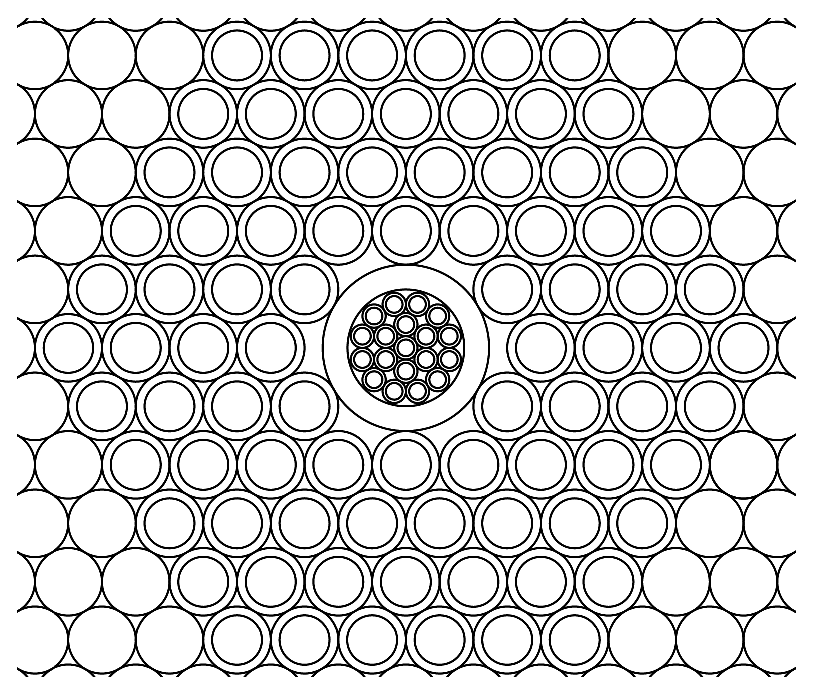
\includegraphics[width=0.48\textwidth]{Pak_build/figs/hexpak_zoom}
    \hfill
    \includegraphics[width=0.48\textwidth]{Pak_build/figs/19fibers}
    \vspace{1.5mm}
    \caption[HexPak Science Fibers]{\fixspacing \emph{Left:} Detail of the
      HexPak science fibers.  Fiber core regions are not shown for packing
      fibers.  The region depicted is approximately 0.18in$\times$0.15in
      centered on the hexagon.  \emph{Right:} Prototype of the HexPak core
      packing.  The fibers and capillary were glued into a 0.25in brass
      ferrule and ground to an even length in order to observe the quality of
      the packing.  This face has not been well-polished and does not
      represent our final target level of surface polish.
    \label{fig:hex_head}}
\end{figure}


The HexPak IFU head is designed to study objects with radial surface
brightness profiles (e.g.\ face-on galaxy disks, spheroidal galaxies).  As the
name suggests, HexPak is a hexagonal fiber array, based on a hexagonal lattice
arrangement.  As a result, the larger-diameter HexPak fibers are arranged in
the most compact manner possible.  The fiber diameter for the hexagonal region
was set by the diameter of the pre-existing DensePak fibers.  These fibers
have core diameters of 310$\mu$m and full outer diameters measured to be
$405\mu$m.  At the plate scale of the WIYN focal plane the cores of these
fibers span 2\farcs8\ on the sky.  The design goal for the HexPak head was to
have a hexagonal region of fibers in an annulus around a high-spatial
resolution fiber core, necessitating two different fiber diameters.  There are
only nine possible compact\footnotemark\ packings of two circle diameters in a
plane \citep{Kennedy06}.  \footnotetext{A packing is ``compact'' if, for every
  circle \emph{C} that is tangent to a series of circles
  \emph{C}$_1$,\emph{C}$_2$,\dots,\emph{C}$_n$, circle \emph{C}$_i$ is tangent
  to circle \emph{C}$_{i+1}$ for $i = 1,2,\dots,n$.}  Of these, only one is
particularly relevant to the science goals of HexPak.  This packing involves
replacing one larger circle with an array of seven smaller circles (with a
diameter ratio of $\sim$0.386) while retaining the hexagonal lattice
arrangement of the other large circles (see Figure~1.e in
Ref.~\citenum{Kennedy06}).


The main flaw in this design as it pertains to our design goals is that the
seven smaller circles \emph{must} be surrounded by larger circles to maintain
a compact packing.  Stated differently, this arrangement dictates that the
high-resolution core of HexPak be no larger than the diameter of one large
fiber.  The reason behind this is that the largest radius occupied by the
seven smaller fibers is larger than the radius of the one fiber which was
removed.  Adjacent packings of seven small fibers would therefore overlap each
other.  This means that this packing arrangement would allow for higher
spatial sampling of no larger than a 2\farcs8\ diameter region, but we felt a
larger region would more closely meet our science goals.  In order to achieve
a larger high-resolution core, we realized that this particular compact
packing can be reversed by instead replacing seven circles with one larger
circle.  This reversal ultimately led to the final design.


For the final HexPak head design we have replaced the central seven
2\farcs8\ fibers in the hexagon with a glass capillary tube.  The outer
diameter of this tube is such that it packs compactly to the surrounding
fibers, and the inner diameter of the tube leaves a large, circular profile in
which we can pack small fibers.  Our final task was to determine how to
densely pack a moderate number of fibers inside this new circular aperture.
In order to determine an efficient packing within this aperture, we once again
turned to the study of circle packing.  A sub-field of circle packing
investigates the most efficient methods for packing circles of a given
diameter into one circle of a larger diameter.  Ref.~\citenum{Kravitz67}
presents empirically-derived optimal packings of circles into a circular
container.  For a diameter ratio of $\sim$0.206, it is possible to pack 19
small circles into one larger circle.  This final design of all the HexPak
object fibers can be seen on the left in Figure~\ref{fig:hex_head}.


It was prohibitively expensive to fabricate a form for a custom diameter
capillary draw just a few inches in length, so in practice our chosen diameter
(and the diameters of the fibers in the core) was limited to stock sizes.  In
the case of HexPak, our chosen glass capillary was purchased from Polymicro
Technologies\footnotemark\ and has a specified inner diameter of 750$\mu$m.
\footnotetext{Polymicro Technologies, 18019 N.\ 25th Avenue, Phoenix, AZ
  85023--1200, (602) 375--4100} This capillary inside diameter corresponds to
a core fiber outer diameter of about 154$\mu$m.  The closest stock fiber outer
diameter from Polymicro was 140$\mu$m (100$\mu$m or 0\farcs94 core diameter),
resulting in the final design of 19 0\farcs94\ fibers packed in the center of
the hexagon.  One sacrifice we make in using stock sizes is that there is a
2--3\arcsec\ gap between the core fibers and the larger fibers in the
hexagonal region.  The necessary outer diameter to fill the space of seven
405$\mu$m OD fibers is 1,050$\mu$m, but this capillary has an outer diameter
of 850$\mu$m.  This amount of undersizing is problematic for the packing
arrangement.  We manually thickened the pieces of capillary used in the head
by applying thin coatings of spray paint to the tubes until we reached the
desired diameter.


\begin{figure}[t]
    \centering
    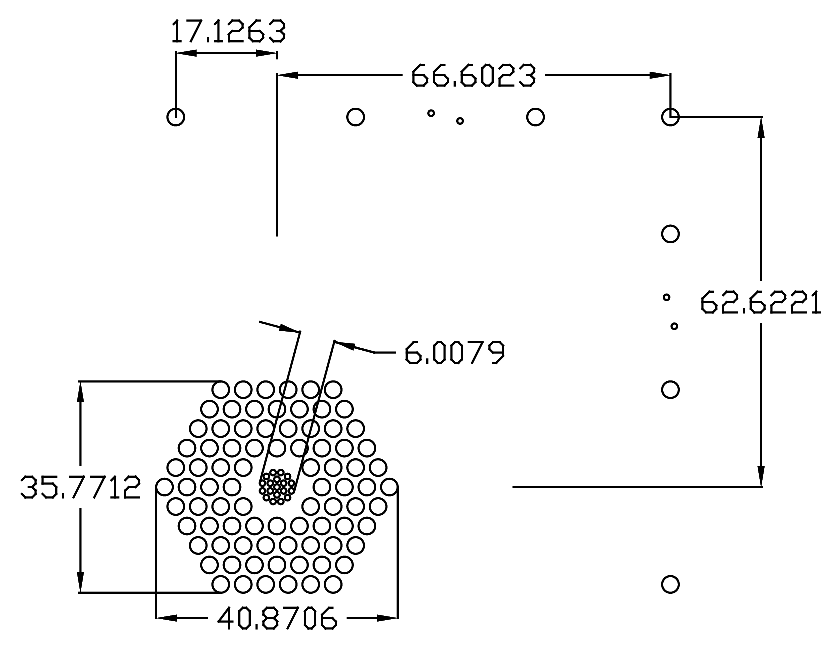
\includegraphics[width=.55\textwidth]{Pak_build/figs/hexpak}
    \hfill
    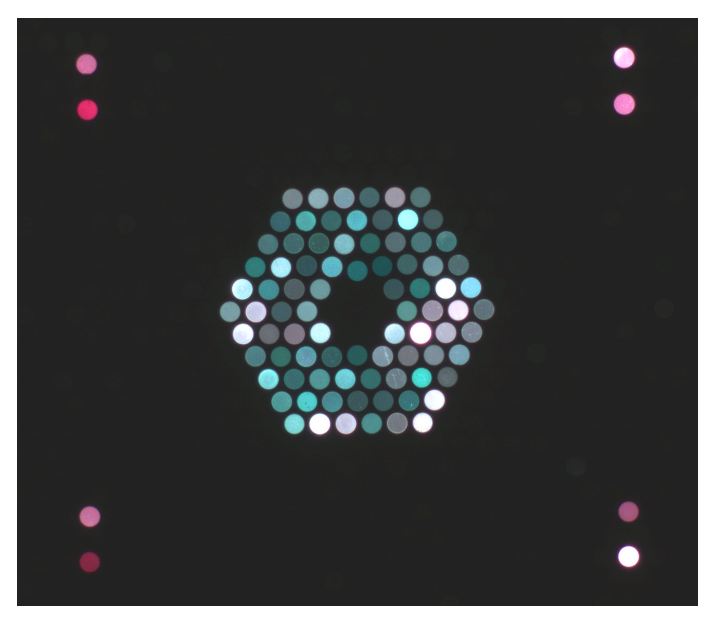
\includegraphics[width=.42\textwidth]{Pak_build/figs/hex_proto}
    \vspace{1.5mm}
    \caption[HexPak Design]{\fixspacing \emph{Left:} Head design for the
      HexPak IFU.  All displayed values are in units of arcseconds.  The two
      different fiber diameters are 2\farcs8 and 0\farcs94 on the sky.  Only
      the active fiber core regions are shown.  \emph{Right:} An image of an
      early prototype of the HexPak head design.  The center of the hexagonal
      region contains a hypodermic needle as a placeholder for the capillary
      with small fibers.  No small fibers are in the hypodermic shown here.
      The ends of the fibers were colored with marker to easily differentiate
      object fibers (green) from sky fibers (red).
    \label{fig:hexpak}}
\end{figure}


Although the results from Ref.~\citenum{Kravitz67} are empirical (and
therefore may not be compact) and our chosen fibers are slightly undersized,
the amount of extra space in the packing arrangement is at an appropriate
level to allow for mechanical tolerances.  We have successfully assembled two
prototypes of this packing and have high confidence that this will be viable
in the final head assembly.  The right side of
Figure~\ref{fig:hex_head} shows one of these prototypes after being
glued and roughly polished.


Our final head design is shown in Figure~\ref{fig:hexpak}.  The array design
has 114 total fibers.  Of these, the main science fiber region consists of 84
fibers with 2\farcs8\ diameters contained within the outer hexagonal region
and 19 fibers with 0\farcs94\ diameters spanning the central
6\arcsec\ diameter of the hexagon.  The capillary tube housing the
0\farcs94\ fibers creates an annular gap 2--3\arcsec in radius between the
core fibers and the outer hexagonal region.  The array also has 11 total sky
fibers, seven with 2\farcs8\ diameters and four with 0\farcs94\ diameters.
The sky fibers are placed along the edges of the array opposite the science
fibers to maximize the separation between the object and sky sampling regions.
The sky fibers lie between 45\arcsec\ and 75\arcsec\ from the \emph{edge} of
the hexagon.  The HexPak head design employs nearly 1,000 short (3in) packing
fibers to fill the space in between the science fibers and the sky fibers,
similar to the scheme used for SparsePak.  The packing fibers also create a
roughly rectangular exterior head profile.  An early prototype of the HexPak
design is also shown in Figure~\ref{fig:hexpak}.  This prototype shows an
earlier revision in sky fiber arrangement and contains no small fibers in the
core of the array.


Ref.~\citenum{Bershady04} found that focal ratio
degradation\footnotemark\ (FRD) increases at the edge of the SparsePak array.
\footnotetext{Focal ratio degradation is a decrease in focal ratio of a beam
  as it passes through a fiber.}  They suggest several possible causes,
including stress incurred when releasing the head from its mold and pressure
introduced by the head-mount clamp.  Regardless of the cause, they recommend
leaving at least a 1.2mm buffer region at the outside of the head in order to
protect the active fibers from these potential stresses.  The ``packing
fiber'' buffer in the HexPak head is four large fibers, or about 1.6mm, which
we expect will alleviate FRD increases at the edge of the array.


\subsubsection{\GP}
\label{GPBsubsub:sec:gradhead}

\begin{figure}[t]
    \centering
    \begin{minipage}[c]{0.5\textwidth}
        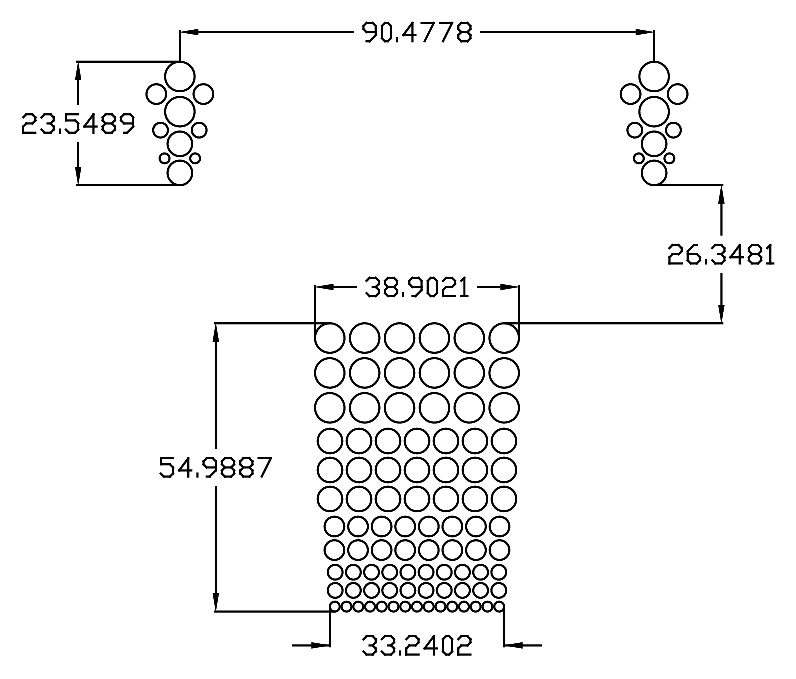
\includegraphics[width=0.95\textwidth]{Pak_build/figs/gradpak}
    \end{minipage}
    \hfill
    \begin{minipage}[c]{0.41\textwidth}
        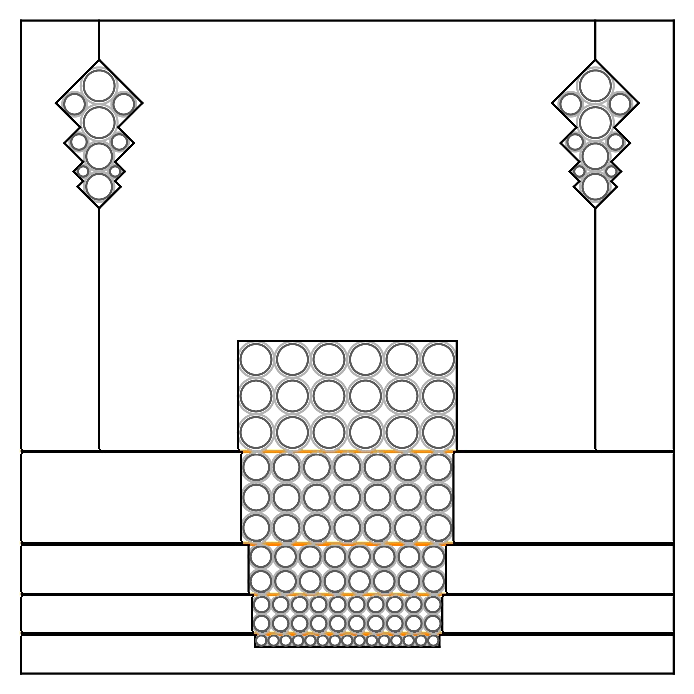
\includegraphics[width=0.95\textwidth]{Pak_build/figs/gradpak_zoom}
    \end{minipage}
    \vspace{1.5mm}
    \caption[\GP Layout]{\fixspacing \emph{Left:} Fiber layout for the \GP
      IFU.  All displayed values are in units of arcseconds.  The different
      fiber diameters are 1\farcs9, 2\farcs8, 3\farcs7, 4\farcs7, and
      5\farcs6 on the sky.  Only the active fiber core regions are shown.
      \emph{Right:} Detail of the \GP head mount.  The darker gray circles
      are the active fiber cores, the lighter gray circles are the full
      O.D.\ of the fibers, and the orange lines represent $25\mu$m-thick
      plastic dividing layers.  The full exterior profile measures
      0.5in$\times$0.5in.
    \label{fig:gradpak}}
\end{figure}


\GP is designed to study objects that exhibit linear gradients in surface
brightness (e.g.\ edge-on galaxy disks, linear outflows).  Therefore, the
desired fiber arrangement in the head is linear rather than approximately
circular as it is in HexPak.  The design goal was to approximate layered
pseudo-slits of increasing slit width, accomplished by using stacked rows of
fiber, with fiber diameters increasing between rows.  There is no compact
packing of two different circle diameters that allows for each fiber size to
be arranged into linear, contiguous rows.  Circle packing theory did not show
obvious solutions for this problem, so we settled on a design that uses five
physically separated fiber regions, each containing only a single fiber
diameter.  This design is shown on the left in Figure~\ref{fig:gradpak}.  Our
final design includes a total of 110 fibers composed of five different fiber
core diameters: 200$\mu$m, 300$\mu$m, 400$\mu$m, 500$\mu$m, and 600$\mu$m.
Respectively, these fibers span angular diameters of 1\farcs9, 2\farcs8,
3\farcs7, 4\farcs7, and 5\farcs6\ at the WIYN focal plane.  In order to
successfully accommodate five different fiber diameters within the same
packing arrangement, we have designed a layered head mount.


This head mount fixturing represents one of the largest engineering challenges
we have overcome.  In order to get each row of fibers to remain parallel to
each other, fibers of different diameters could not touch.  This is a result
of there being no compact packing of two different fiber diameters that allows
for parallel rows.  This meant that it would be impossible to use short
packing fibers in the \GP head.  After numerous iterations, we ultimately
designed a layered head mount that is assembled in stages, one fiber-diameter
region at a time.  The final head mount design can be seen on the right in
Figure~\ref{fig:gradpak}.  Each set of fibers of a given diameter is contained
by aluminum walls, precisely machined to the height of each fiber region.  The
head is then assembled by layering subsequent stacks of these segments on top
of one another.  All of the parts of the fixture are held together as an
assembly using small dowel pins that run the full height and width of the
assembly.  The main cavity was cut out as an assembly using a wire electric
discharge machining (EDM) process to ensure the best possible alignment
between adjacent fiber regions.  The \GP head block cavity was cut using a
0.004in diameter wire, allowing for a minimum corner radius of 0.002in
(50$\mu$m), small enough to ensure the smallest fibers fit into place.

The dimensions of the entire head block are 0.5in$\times$0.5in.  Each region
of fibers containing a single fiber diameter is separated from its neighbors
by a thin layer of plastic shim stock 0.001in (25.4$\mu$m) thick.  Although
this adds a gap between each region of fibers, the on-sky angular size of the
plastic layer is very small (0\farcs24), which we deemed acceptable.  We have
successfully designed and assembled two prototype \GP head assemblies and
we are confident that this design is feasible.


The resulting array design consists of five stacked blocks of fibers arranged
into one or more rows, with the fiber core diameter increasing from 200$\mu$m
to 600$\mu$m between each block of fibers.  The entire block of science fibers
includes 90 fibers and covers an area on the sky roughly
35\arcsec$\times$55\arcsec.  The array also has two regions of sky fibers for
simultaneous sky measurements.  Each sky fiber region contains two fibers of
each fiber diameter included in the science fiber region.  The fibers in
\GP are arranged in a square lattice rather than in a hexagonal lattice,
reducing the effective filling factor within each fiber region.  This yields a
packing density of only $\pi/4 \approx 0.785$.  The advantage of this
arrangement is that the pseudo-slits within each region are vertically aligned
and are offset only in one dimension on the sky.


Since the entire \GP head mount assembly is composed of aluminum parts, no
short packing fibers are used in its design.  The design does, however, place
active fibers within 1.2mm of the edge of the head, inside the prescribed
minimum buffer distance.  However, we believe FRD edge effects should be
negligible due to the use of a stronger buffer material (aluminum in this
case) and the fact that at no point during assembly is any part of the \GP
head released from a mold.


%%%%%%%%%%%%%%%%%%%%%%%%%%%%%%%%%%%%%%%%%%%%%%%%%%%%%%%%%%%%%
\subsection{Slit design} 
\label{GPBsub:sec:slit}

\GP and HexPak both terminate in the same ``foot'' housing in a dual-slit
configuration.  The slit block uses a custom design that modified the
SparsePak slit block design.  The slit block assembly is made from two
separate aluminum plates, each specifically designed to create a pseudo-slit
for one of the IFUs.  Each pseudo-slit was created by cutting `v'-grooves into
the slit block.  The groove size, placement, and spacing is designed to match
the varying number and sizes of fibers in each IFU pseudo-slit.  A schematic
of the slit block assembly is shown in Figure~\ref{fig:slit}.  For mechanical
reasons, the fibers are aligned to be tangent to the optical center line of the
slit, rather than being aligned by their centers.  The `v'-grooves were
precision-cut into the slit block using a wire EDM process like that used for
the \GP head mount fiber cavity, but with a smaller $0.002$in diameter
wire, resulting in a minimum corner radius of approximately $0.001$in
($25\mu$m).  This radius is smaller than the smallest fiber outer radius
(measured to be about 71$\mu$m) ensuring that even the smallest fibers will
sit nicely into the grooves.


We have set the fiber core edge-to-edge spacing at $291\mu$m to minimize
cross-talk while maximizing the number of fibers in the slit.
Ref.~\citenum{Bershady04} found that 400$\mu$m was the ideal edge-to-edge
spacing of fiber cores in the slit in terms of the trade-off between
cross-talk and packing density (i.e.\ total number of fibers).  However, this
determination was made using the old Bench Spectrograph system which was
upgraded in 2008 \citep{Bershady08}.  With improved image quality and detector
sampling as a result of the upgrade, we estimate we can reduce the fiber
spacing by $\sim25\%$ without introducing significant amounts of cross-talk
between fiber channels.


The fiber arrangements in the slit are informed by their locations within the
head design.  In HexPak, the hexagonal region is divided into six equal
wedges, each containing 14 fibers.  The fibers within each wedge are located
in the same region of the slit, with fibers near the core of the array being
located in the center of the slit segment.  Each wedge section in the slit is
separated from the adjacent wedge sections by a sky fiber, allowing sky
sampling across the entire slit length.  Three wedges and associated sky
fibers are located on each end of the slit, separated by all of the 0\farcs94
fibers.  The 0\farcs94 fibers are located in the center of the slit, with the
associated 0\farcs94 sky fibers being located on either side of the
0\farcs94 object fibers.  The \GP slit is sorted by fiber diameter.
Within each diameter region, each fiber row in the head is placed contiguously
in the slit, with sky fibers evenly distributed as separators between rows.


We also slightly modified the standard Bench Upgrade design for the ``toes''
of the cable in order to negate vignetting of the light exiting the fiber
slit.  The toes house the slit block and have open chambers for inserting
blocking filters, slit masks, and a back-illumination mirror.  These chambers
each have an aperture through which the exit beam must pass in order to reach
the spectrograph collimator.  We performed a vignetting analysis to determine
the maximum fiber slit width and slit length that could pass unvignetted
through the toes.  Ref.~\citenum{Bershady04} shows that, due to FRD, 99\% of
the energy in an \f6.3 input beam (the WIYN focal ratio) exiting the fibers is
contained within an \f4 output beam.  Therefore, as long as an \f4 beam could
pass through the toes without being blocked, we could consider light losses
from the toes to be negligible.  The SparsePak design for the toes allowed for
a maximum slit length of 79.8mm under this vignetting requirement.  This
number informed the fiber-to-fiber spacing for our final slit design,
resulting in an overall slit length of 76.6mm.  The maximum allowable slit
width for an \f4 beam was 1.23mm, or a $615\mu$m beam displacement from slit
center.  Our largest fiber has a $600\mu$m core diameter with approximately
$55\mu$m of cladding and buffer in radius.  Each half of the slit block also
has a $25\mu$m plastic divider at slit center, a requirement of our slit block
construction process.  In total, the maximum beam displacement from slit
center is about $680\mu$m, too large for the standard design for the toes.  As
a result, we modified the design and increased the width of one critical
aperture in the toes such that the maximum allowable displacement from slit
center is $927\mu$m.


\begin{figure}[t]
    \centering
    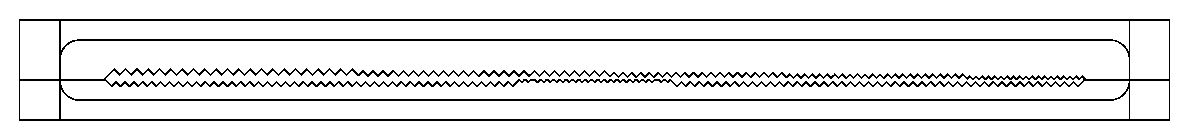
\includegraphics[width=\textwidth]{Pak_build/figs/slit}\\
    \vspace{2pt}
    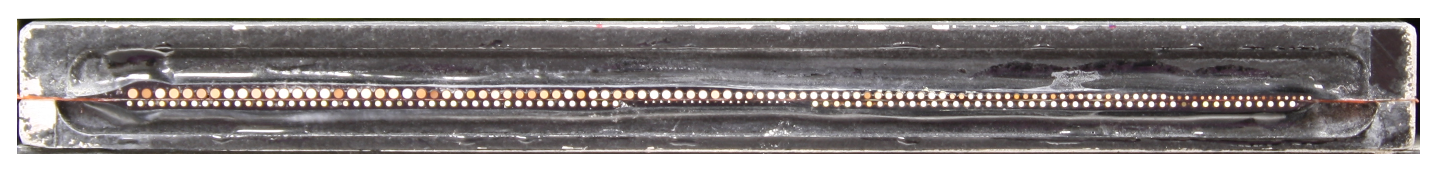
\includegraphics[width=\textwidth]{Pak_build/figs/slit_img}
    \caption[HexPak/\GP slit]{\fixspacing \emph{Top:} A schematic view of the
      slit block without fibers.  Both halves of the slit block assembly are
      shown.  The bottom set of grooves is the HexPak slit and the upper set
      of grooves is the \GP slit.  \emph{Bottom:} An image of the slit
      face in its current state.  The top row of fibers are \GP, arranged
      by decreasing diameters.  The bottom row of fibers are HexPak, with the
      0\farcs94 fibers situated between the 2\farcs8 fibers.  Brightness
      differences between fibers are largely due to surface irregularities in
      the unpolished head end.  Color differences are simply due to some
      fibers pointing at different parts of the lab.  The two 0.001in-thick
      plastic shim stock dividers are seen as a thin orange line separating
      the two slits.  The shown view spans 3.562in$\times$0.312in.
    \label{fig:slit}}
\end{figure}


%%%%%%%%%%%%%%%%%%%%%%%%%%%%%%%%%%%%%%%%%%%%%%%%%%%%%%%%%%%%%
\section{Construction and Status} 
\label{GPB:sec:construction}

The design and construction of the SparsePak cable served as the starting
point for this instrument.  Technical details of SparsePak fabrication are
available in the Appendix section of Ref.~\citenum{Bershady04}.  In this
section we focus primarily on detailing the important features unique to this
instrument and noting significant departures from the SparsePak design.


At the present time, construction is complete on all cabling and the entire
spectrograph feed assembly (the foot).  Polishing of the fiber slit is nearly
complete, and final gluing and polishing of the IFU heads are scheduled to
conclude in June--August 2012.

\subsection{Fiber optics}
\label{GPBsub:sec:fibers}
The 91 2\farcs8\ fibers that compose the hexagonal region and its associated
sky fibers are re-purposed from the DensePak IFU.  They have a specified
active core diameter of $310\mu$m and a measured total O.D.\ (including
cladding and buffer) of approximately $405\mu$m.  Ref.~\citenum{Barden98}
states that the DensePak fibers are similar to the Hydra FIP-type
``red-optimized'' fibers.  The 23 0\farcs94\ fibers forming the
high-resolution core and associated sky fibers were purchased new from
Polymicro Technologies.  These new fibers are FBP-type broad-spectrum optical
fiber with excellent throughput for optical wavelengths.  The fibers have
silica cores with silica cladding and are designed to have excellent
throughput across the visible spectral window and into the near-infrared.  The
diameter specification (given as core:clad:buffer, in microns) is 100:120:140.
This new fiber is very similar to the fiber used in SparsePak and therefore we
expect similar throughput performance from the core HexPak fibers.

Throughput testing for SparsePak showed a roughly 20\% improvement in
throughput compared to the DensePak fibers, after accounting for differences
in fiber diameter and collected solid angle \citep{Bershady05}.  However, most
of the light loss in the DensePak cable was likely due to vignetting in the
original design of the fiber cable toes, before the Bench Upgrade.  With our
modified version of the standard Bench Upgrade toes, we expect these fibers to
have comparable performance to the SparsePak fibers in the red ($>4000$\AA;
the FBP-type fibers have better transmission properties below
4000\AA\ compared to the FIP-type fibers).

The \GP IFU consists entirely of new FBP-type broad-spectrum optical fiber
from Polymicro Technologies.  The fibers have specified diameters (given as
core:clad:buffer, in microns) of 200:220:240, 300:330:370, 400:440:480,
500:550:590, and 600:660:710.  This fiber is very similar to the fiber used in
SparsePak and therefore we expect similar throughput performance from all the
\GP fibers.


\subsection{Cabling}
\label{GPBsub:sec:cabling}
Each fiber is individually housed in a PTFE tube for protection and strain
relief.  The PTFE tubes for the $310\mu$m HexPak fibers were also re-used from
the DensePak cable.  All of the newly-purchased fiber is housed in new PTFE
tubing from Zeus, Inc\footnotemark.  \footnotetext{Zeus, Inc., 3737 Industrial
  Blvd., Orangeburg, SC 29118, (800) 526--3842} As a design decision to reduce
the radial cable size, the new PTFE tubes have ``light-weight wall''
thicknesses (0.006in in radius).  This has proven troublesome due to the
relative lack of radial strength and rigidity in the wall compared to
thicker-walled tubing.  The very thin walls of these tubes are prone to
kinking which threatens the integrity of the fibers they serve to protect.  We
recommend, at minimum, ``thin wall'' PTFE tubes ($\gtrsim$0.01in).


The PTFE tubes terminate at each end of the cable in metal shear clamps.  The
foot-end shear clamp contains an array of approximately $9\times27$ holes in a
three-element aluminum clamp.  The elongated design of this clamp serves to
transform the circular bundle of fibers into a rectangular shape approximating
the slit arrangement.  The head-end shear clamps are a similar three-element
design and function in a similar fashion to the foot shear clamp.  The hole
pattern in the head end shear clamps is roughly hexagonal in order to
accommodate the circular fiber bundle and to approximate the fiber layout of
the HexPak head.


The fibers and their PTFE tubes are encased in 75 feet of flexible metal
conduit.  The conduit housing the shared length of the cable consists of
approximately 57 feet of 2in ID IE30 and IE50\footnotemark\ interlocking
stainless steel exhaust hose.  \footnotetext{Penflex, Corp., 105B Industrial
  Drive, Gilbertsville, PA 19525, (800) 232--3539} This conduit retains
flexibility for handling while providing strength and durability for the
length of cable that will be enclosed within the telescope structure.


The remaining 18 feet of the cable is housed in two separate lengths of 1.25in
ID flexible aluminum standard electrical conduit.  Each length contains the
remaining length of fiber for one of the IFU heads.  The lightweight
construction and smaller diameter of this conduit allows for ease of handling
for mounting the IFU heads into the telescope's Nasmyth port.  These two
lengths of conduit are completely covered in polyolefin and PVC heat-shrink
tubing for additional rigidity and abrasion resistance.  The smaller lengths
of conduit are joined to the larger, stainless steel conduit through a
custom-built merge collector from the automotive industry\footnotemark.
\footnotetext{Specialty Design Products, Inc., 11252 Sunco Drive, Rancho
  Cordova, CA 95742, (888) 778--3312}


The conduit for each IFU head contains two custom-designed low-profile
rotation couplers.  Each coupler has $180^{\circ}$ of rotation about the
optical axis, allowing each IFU head to rotate a full $360^{\circ}$ with the
telescope instrument port rotator.  The two rotation couplers are spaced
approximately $12$in apart along the cable to ensure that the full rotation is
distributed along a sufficient length to avoid fiber stress.


\subsection{Fiber slit}
\label{GPBsub:sec:slitconstruct}
For gluing the fiber ends into the slit grooves, we fabricated custom metal
fixturing to bend the fibers 90$^{\circ}$ in the foot and hold them with
clearance to mount the slit blocks.  We used EPO-TEK\footnotemark\ 354
heat-curing optical epoxy to bond the fiber ends to the slit block.
\footnotetext{Epoxy Technology, Inc., 14 Fortune Drive, Billerica, MA 01821,
  (978) 667--3805} The gluing fixture held each fiber in its respective slit
position and allowed us to seat all the fibers simultaneously.  We used a thin
sheet of plastic to cover the exposed fiber and epoxy and held the fibers in
place using an aluminum pressing block while the epoxy cured.  We glued each
slit block separately and then constructed the final assembly from the two
completed halves.  The two halves are pinned together to ensure accurate,
repeatable positioning between the two slit halves.

\subsection{Fiber heads}
\label{subsec:headconstruct}
As tested with SparsePak and our HexPak and \GP test head assemblies, we
will use the same EPO-TEK 354 heat curing epoxy for assembling the IFU heads.
The HexPak head is assembled one row of fibers at a time, using short packing
fibers to fill in the spaces around the active fibers.  The 0\farcs94\ fibers
are pre-assembled into their capillary tubes and then placed into the final
assembly during the gluing process.  For constructing the HexPak head, we
follow a design and process used for SparsePak, based on a concept from
S.\ Barden (\emph{private communication}).  We will assemble the fibers in a
micrometer-driven vice with the vice channel width set precisely to the width
of the head.  We will then use a precisely-machined tamping tool, just
slightly narrower than the width of the head, to pack the fibers into the
channel mold.  The mold and the tamping tool are sprayed with a PTFE mold
release\footnotemark[1]\ prior to gluing.  \footnotetext[1]{Miller--Stephenson
  Chemical Company, Inc., 55 Backus Ave., Danbury, CT 06810, (203) 743--4447}


The \GP head is assembled one fiber region at a time, with all fibers of a
single diameter being assembled at the same time.  The assembly is cured after
each additional region is assembled.  In contrast to the HexPak construction,
no vice is used for \GP.  The head mount parts are machined to the precise
cavity width to hold the fibers for each region, requiring only a pressing
plate to ensure the fibers remain seated in the cavity while curing.  The
pressing plate is coated in PTFE mold release as a precaution and separated
entirely from the epoxy by the plastic dividing layers, so at no point are the
fibers released from a cured mold.  This should alleviate any additional FRD
introduced through fiber stresses when releasing the mold, as seen in
SparsePak.


%%%%%%%%%%%%%%%%%%%%%%%%%%%%%%%%%%%%%%%%%%%%%%%%%%%%%%%%%%%%%
\subsection{Polishing}
\label{subsec:polishing}
We will polish the optical surfaces of the fiber slit and each of the fiber
heads in order to minimize light losses and FRD as the light passes through
the cable.  We are using an UltraPol\footnotemark[2]\ 1200 model lapping
machine with 8in diameter silicon carbide and aluminum oxide lapping disks.
\footnotetext[2]{ULTRA TEC Manufacturing, Inc., 1025 E.\ Chestnut Avenue,
  Santa Ana, CA 92701, (877) 542--0609} The lapping disks span a range of grit
sizes, starting from $70\mu$m for the grinding phase to $0.3\mu$m for the
final polishing phase.  Our laboratory testing shows that FRD is minimized for
surface roughness $<5\mu$m.  Our target surface roughness is $<0.5\mu$m.
See Eigenbrot et al.\ in these proceedings for a full description of our FRD
and surface polish testing.  At the time of this writing, the entirety of the
slit was polished at a 5$\mu$m level and ready to proceed to 1$\mu$m grit
disks, followed by 0.3$\mu$m grit.  An image of the slit in this state is
shown in Figure~\ref{fig:slit}.


%%%%%%%%%%%%%%%%%%%%%%%%%%%%%%%%%%%%%%%%%%%%%%%%%%%%%%%%%%%%%
\section{Summary} 
\label{GPB:sec:conclusion}

We are in the final construction phase of two new fiber optic IFUs, \GP
and HexPak.  These IFUs will be the first formatted fiber IFUs to utilize
multiple fiber diameters within the same IFU head.  By including multiple
fiber diameters these IFUs will greatly expand the spectroscopic capabilities
of the WIYN 3.5m telescope, providing the ability to sample varying spatial
scales within the same observation with the highly versatile Bench
Spectrograph.  This will enable observations simultaneously spanning a wide
range in surface brightness to be optimized for the photon limit at spectral
resolutions between 1000 $< \lambda/\Delta\lambda <$ 30,000.


HexPak is designed to observe axi-symmetric surface brightness profiles with a
$36\arcsec\times41\arcsec$ hexagonal region sampled by 2\farcs8\ fibers and a
6\arcsec diameter high-resolution core sampled by 0\farcs94\ fibers.  \GP
is optimized for linear surface brightness gradients, with a stacked
pseudo-slit design spanning $39\arcsec\times55\arcsec$ using fibers ranging
from 1\farcs9\ to 5\farcs6\ in diameter.  Each of these IFUs presented
unique challenges for successfully incorporating multiple fiber diameters
within the same fiber head.  We have described two methods for overcoming
these challenges, one for radial arrangements of fibers and one for linear
arrangements.  Our solutions optimize the packing fraction of science fibers
while also achieving regular and precise placement and configuration of fibers
within each IFU.

\bibliographystyle{thesis}
\bibliography{Pak_build}
